\chapter{Evaluation}
\label{sec:evaluation}
This chapter presents the evaluation results of the thesis. After some
remarks about the evaluation context in \refsec{sec:eval-context}, we
analyze the durations of different robot memory operations in
\refsec{sec:op-durations}. This includes comparing the durations for
different expressiveness levels and database sizes to find a
compromise between expressiveness and performance. Furthermore, we
analyze the overhead of database operations introduced by robot memory
features. In \refsec{sec:performance} we present the performance of
the system in the already introduced application scenarios. This
includes CPU and memory usage, network throughput, and statistics
about robot memory operations. Qualitatively, we evaluate how well the
features of the robot memory work, how it can support the development
of application scenarios, and where limitations are. Furthermore, we
present experiments regarding the compromise of expressiveness and
performance. \todo[inline]{review mentioning of all sections}

\section{Evaluation context}
\label{sec:eval-context}
The benchmarks presented in this chapter were performed on Fedora 23
systems with 16 GB RAM and an Intel Core i7-3770 with eight cores at
$3.4$~Ghz. For local benchmarks everything, including Fawkes, Mongodb,
the Gazebo simulation and ROS, ran on a single system. For distributed
benchmarks, three identical systems were used. Each system hosted its
own Fawkes, ROS, and Mongodb processes and one system additionally,
hosts the Gazebo simulation.

Since the robot memory runs inside the Fawkes framework and thus
inside the Fawkes process, the performance of the robot memory can not
directly be measured separately and is influenced by Fawkes. The
influences are caused by other components, such as localization,
reasoning, and collision avoidance, and by the thread management of
Fawkes. To softly guarantee loop times for other threads, Fawkes
suspends threads with a too long loop iteration. When measureing
durations of robot memory operations, this can increase large
measurement values because if an operation takes longer than the
allowed loop iteration time, the time being suspended is added to the
measurement.

\section{Robot Memory Operations}
\label{sec:op-durations}
In this section, we analyze the run-time durations of robot memory
operations, such as insert, query, and update. We also analyze how
these change with computables and triggers. The goal is to find out
how fast the robot memory works. Besides the influence of the
implementation, the durations heavily depend on the underlying
complexity (e.g. of a query) and \emph{domain size}, which is the
amount of information stored in the robot memory. Here, we want to
find out how the durations scale with increasing domain size and
increasing complexity.

The structure of the data used for this evaluation is chosen in a way
that it is similar to information that is usually stored in a robot
memory and that it also simplifies the analysis. The used data mimics
a robot's knowledge about object and their positions to solve a tidy
up scenario. For each object, the robot memory contains a document
with the object's name, current position, and the storage position it
belongs to. Names are unique and storage positions are randomly chosen
out of $1000$ possibilities. Objects are currently placed at their
storage position with probability $0.05$ and random otherwise. The
object's name is string to enforce string comparisons, which are
expected to be often needed in a real scenario. For evaluation
reasons, we do not index the collection by the s name right now
because this heavily impacts the duration. An evaluation plugin in
Fawkes generates the data and calls random operations. To analyze how
the durations scale with the domain size, the plugin calls the
operations repeatedly after increasing the domain size from $0$ to
$100000$ documents by steps of $1000$ documents.

The analysis is separated into the main classes of operations, namely
insertions in \refsec{sec:insertions}, queries in
\refsec{sec:queries}, and updates in \refsec{sec:updates}. Because
deletions behave very similar to updates, both search for documents
and work with them, they are also covered in the section about
updates. \refsec{sec:eval-computables} covers and explains the impact
of computables on query durations and \refsec{sec:eval-trigger} deals
with the impact of event triggers. Operations that are performed
rarely are not analyzed. For example dropping or restoring a collection and
registration of triggers and computables are only performed once
during initialization.  In the course of implementing and evaluating
the application scenarios, their durations were not noticible compared
to the initialization time of the whole robot software.

\subsection{Insertions}
\label{sec:insertions}
\begin{figure}
  \centering
  \begin{subfigure}[b]{0.5\textwidth}
    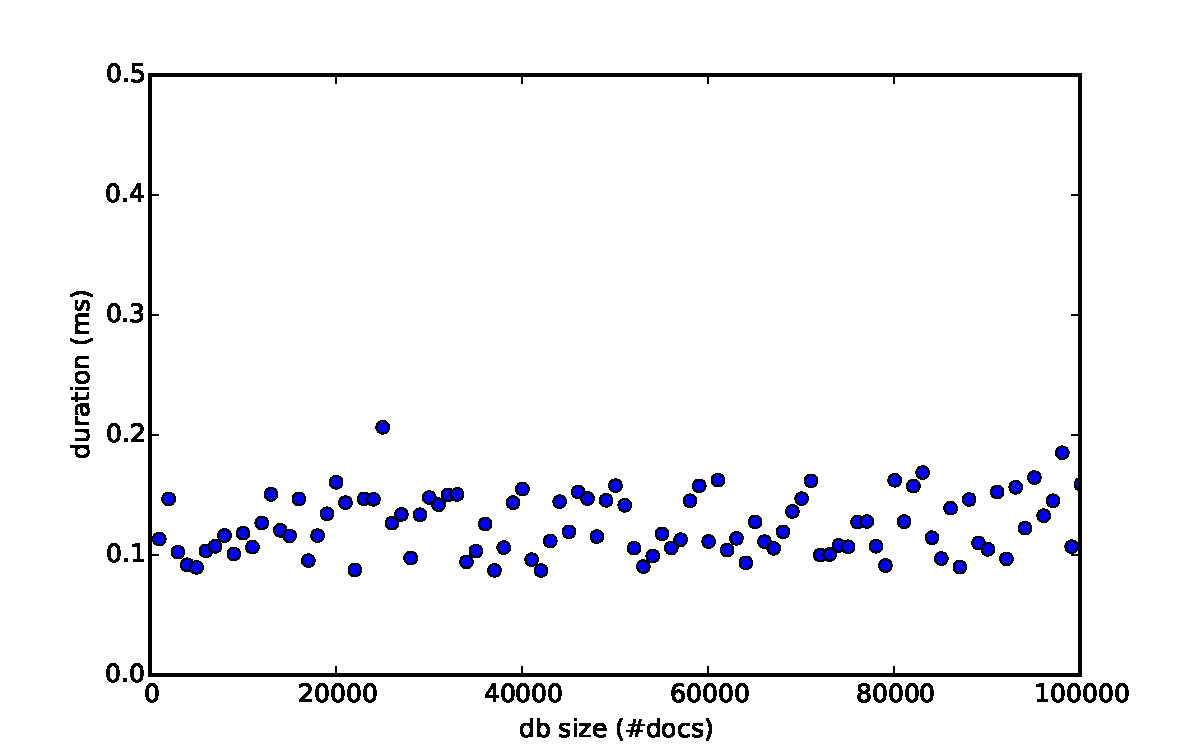
\includegraphics[width=\textwidth]{plots/insert-durations}
    \caption{Insertions}
    \label{fig:insert-durations}
  \end{subfigure}
  \begin{subfigure}[b]{0.5\textwidth}
    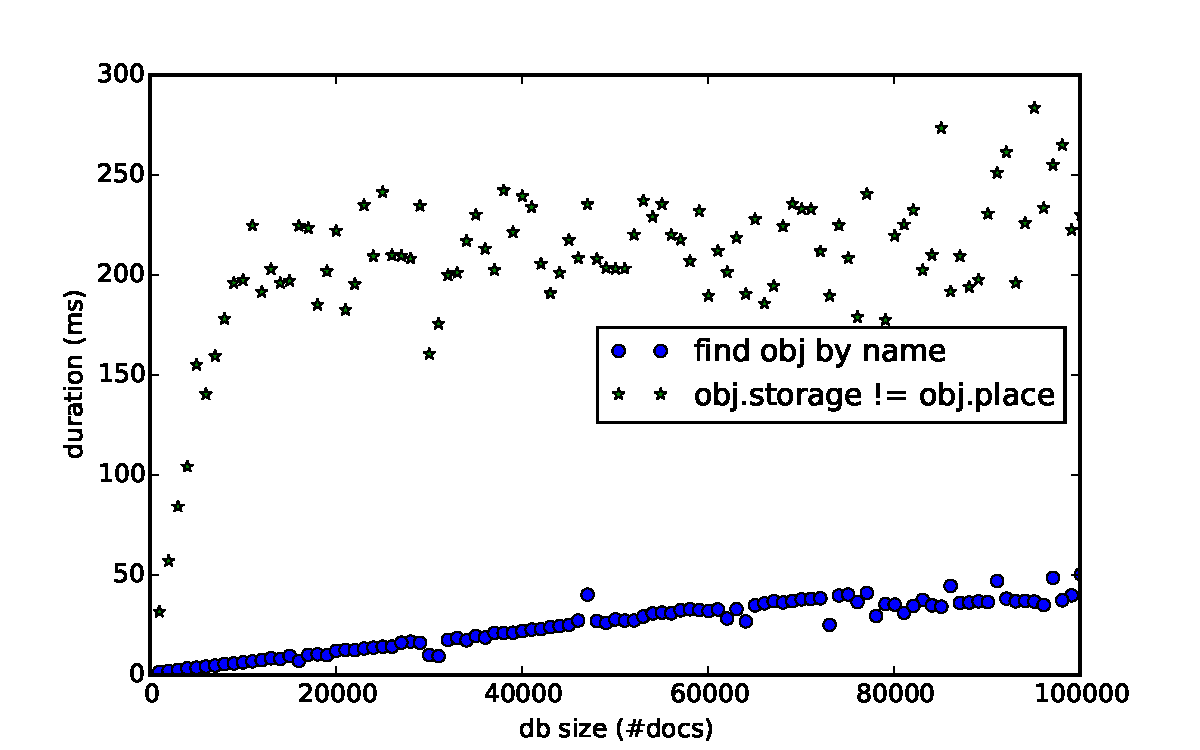
\includegraphics[width=\textwidth]{plots/query-durations}
    \caption{Queries}
    \label{fig:query-durations}
  \end{subfigure}
  \caption[Duration of insert operations with increasing domain size]{Duration of robot memory operations with increasing domain size}
  \label{fig:eval-durations-1}
\end{figure}
The insertion of a new document into the robot memory is overall the
fastest operation compared to queries and
updates. \reffig{fig:insert-durations} shows the distribution of
insert durations with increasing domain size. It is noticible that the
duration does not depend on the domain size and thus has run-time
complexity of $O(1)$. The insertion time is small with an average of
$0.125ms$. However, there are single outliers not present in
\reffig{fig:insert-durations}. These outliers occur periodicly, when
MongoDB flushes database changes from the RAM to the hard drive. We
could reduce frequency of these outliers to one in $60s$, which is the
default flushing frequency of MongoDB. To reach this, we had to
disable the forward logging of MongoDB, called Journaling. In this
evaluation scenario, the outliers took about $0.3s$ because of the
large amount of written documents and the threading in Fawkes.  The
overhead of the robot memory compared to the duration of the raw
MongoDB operation has an average of $0.006ms$, which is about $5.5\%$.
The overhead is caused by verifying the collection name, deciding if
the local or distributed database is used, and adding meta-data.  The
robot memory overhead mesured here does not include checking if
triggers were activated by inserting the document. This is caused by
the asynchron and seperate checking by the trigger manager. The size
and the complexity of insertes documnents did not make a noticable
difference.\todo{nedd to add numbers?}

\subsection{Queries}
\label{sec:queries}
batch query
(comparison find only one/find all)
overhead
\todo[inline]{comparison with indexing}
performance-size-expressiveness
scale liniar/quadratic with size

\subsection{Updates}
\label{sec:updates}
also includes removes
overhead
performance-size-expressiveness
scale liniar/quadratic with size


\subsection{Computables}
\label{sec:eval-computables}
overhead
performance-size-expressiveness
scale liniar/quadratic with size
\subsection{Trigger}
\label{sec:eval-trigger}
overhead
performance-size-expressiveness
scale liniar/quadratic with size


\section{Performance in evaluation scenarios}
\label{sec:performance}

data scenario: arm, rcll

\section{Qualitative Evaluation}
\todo[inline]{refine qualitative structure}